%\section{Alternative methods for pain treatment}
%Alternative methods for treating pain not involving medication is being explored in the aid of treating patients without risking the side effects of taking medication. The alternative methods of Chiropractic therapy, acupuncture, yoga,  massage therapy, hypnosis, biofeedback and mindfulness meditation will be presented and discussed in the following sections. 

\subsection{Chiropractor}
Adjustment and manipulation of the spinal cord to alignment the vertebrae of the spine to reduce pressure on the nerves running down the spine. \cite{Gerald2013}
In a study by \cite{Peterson2012} evaluating 506 patients with acute and chronic back pain after 3 month of chiropractic treatment.
Patients undergoing chiropractic treatment showed improvements in their condition and the effect was ongoing after 3 month. \cite{Peterson2012}

\subsection{Acupuncture}
Acupuncture is a treatment where small sterile needles are inserted into the skin of the patient. The needles are inserted at specific acupuncture points related to the type of pain that the patient is experiencing. \cite{Dhanani2011} 
In a study by \cite{Junnilla1983} acupuncture has shown promising results in reducing pain in patients with soft tissue round the shoulder joint, headaches, neck and shoulder pain, arthritis/osteoarthritis and low vack pain. A total of 348 patients where evaluated. The mean reduction of the entire patient group where 68 \%. Showing best results in soft tissue round the shoulder joint, showin a mean reduction of pain by 79 \%. The headache and neck and shoulder patients had a mean reduction by 74 \%. Patients with  arthritis/osteoarthritis showed a mean reduction by 58 \% and the patients with low back pain had a mean reduction by 50 \%. In 80 \% of the patients the effect of the treatment lasted for more than 3 month and 32 \% over one year. \cite{Junnilla1983}
% maybe one of these citeations are to old? 

\subsection{Hypnosis}
%Noxious stimuli increased cerebral blood flow in specific areas of the brain in pain processing,  a the thalamic nuclei anterior cingulate and insular cortices.
Hypnosis is a process where the one comes into the state of trance and feels deep relaxation and is open to conversation verbally. Hypnosis is a guided process and can be carried out alone or by others. \cite{Gerald2013} Factors as anxiety, depression and other states of mood and the general the social life of the patient has been shown to play a role in chronic pain. these mechanisms might be altered by hypnosis.
In the literature hypnosis has shown positive to relieve pain, but only on a short term basis. \cite{Dhanani2011}
\fxnote{maybe a bit more text here?}

\subsection{Yoga}
Yoga is a form of mind to body practice discipline, or tradition originating from India. In the practice of yoga different physical postures, breathing techniques and more are the routine. 
Yoga is both a form of personal evolution, but most popular because of the exercise which benefits the health.
A review by \cite{Whitehead2017} found that yoga could improve the functionality of the back and a slight effect of treating pain compared to non-yoga participants. 
\fxnote{Maybe a bit more text here?}
%\subsection{\}Exercise} 

\subsection{Mindfulness meditation}
Mindfulness is often defined as being in the mental state of Non-Elaborative, non-judgmental awareness \cite{Zeidan2012,Zeidan2016,Tang2017}. 
Mindfulness is viewed upon as a lifestyle and the lifestyle of mindfulness can be practiced through meditation, called mindfulness meditation. Practicing mindfulness meditation includes control over sensory, emotional and cognitive happenings. Hereby the ability to control these sensations without being distracted by them as so the ability to abstract from past and future representations of memory. Hereby one can say that mindfulness meditation is training of the mind. \cite{Tang2017}


(.....MAYBE WE NEED SOME KIND OF REASONING TO WHY WE CHOOSE TO LOOK INTO MINDFULNESS MEDITATION, LIKE A SUMMARY OF ALL THE METHODS BEFORE GOING INTO MINDFULNESS MEDITATION, AND THEN DIG DEEPER INTO THE FACTS OF MINDFULNESS MEDITATION....)



Two popular practices of mindfulness meditation, focused attention (FA) and open monitoring (OM) are of the most well practiced types of meditation. \cite{Zeidan2016}

\subsubsection{Focused attention} 
FA is the training of concentration, where one keeps his or her focus at an object or specific thing, only focusing on that thing. Often the flow of breath is the focus, when practicing FA meditation.  When any disturbance comes by, like a thought, sound or other environmental distractions, which will often lead to a drift in attention, the person should always bring his or her attention back to the focus. \cite{Zeidan2016}

This kind of meditation has shown to enhance focus and concentration. ..

\subsubsection{Open monitoring}
OM is the cultivation of open presence, were the mind is open to anything, not focusing on any specific thing, just being in the present. If any thought or disturbance comes by, the thought or sensation should be noticed briefly, but then left without thinking more over it. It is believed that this form of meditation is easier to learn when the person masters the meditation of FA, whereby the OM form is easier to master. \cite{Zeidan2016}

This kind of meditation has been shown to reduce pain more compared to FA, likely because the areas of the brain affected during this form of meditation is...\cite{Perlman2010}

FA and OM can alter pain in different ways...
OM is more effective in reducing pain after extensive meditation training compared to FA. 
\cite{Varilly2012}

\subsubsection{Mechanisms of mindfulness meditation}
Enhanced emotion regulation, cognitive control, acceptance and positive mood have been linked with health benefits as well as pain modulation. These mechanisms has been shown to be modulated during mindfulness meditation practice.
A study by Perlman et al. (\cite{Perlman2010}) shows that practicing meditation could not lower the intensity of pain, but instead lower pain unpleasantness in the participants. \cite{Zeidan2012, Perlman2010}

The typical response when using a placebo analgesia is increased activation of the dorselateral prefrontal cortex during pain anticipation. Effect that predicts reductions in pain perception and activaty of pain related brain regions. Mindfulness meditation does not involve dorselateral prefrontal cortex activation. \cite{Zeidan2012}

The findings on mindfulness meditation and pain modulation are split, but experiments in controlled settings are still needed to confirm if the effect of mindfulness meditation works on pain modulation. \cite{Zeidan2012, Perlman2010}

%\fxnote{....and then we need something like: or maybe a summary of all the methods and then saying, because of this and this, mindfulness meditation will be looked further upon as method for reliving pain...}

%The method of mindfulness meditation will be used for method to relief pain in this project.

%\section{Mindfulness meditation}
%Definition
Different brain regions is involved the practice of mindfulness meditation. The most important are the prefrontal cortex (PFC), involving the anterior cingulate cortex (ACC) and the medial PFC. The striatum, the insula and the default mode network (DMN), which include the medial PFC and the posterior cingulate cortex (PCC). These regions play a big role in the effect of mindfulness meditation and are highly regulating the mechnisms of meditation which can generally be catergorised into the three catagories, attention control, emotion regulation and self-awareness. 

Figure \ref{fig:brain_meditation} shows an image of the brain and the regions involved in attention, emotion and self awareness. 

\begin{figure}[H]
	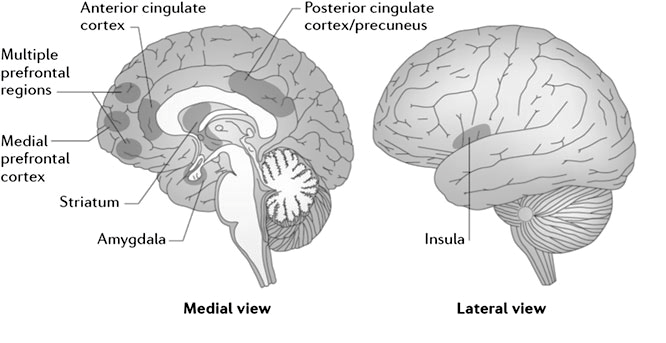
\includegraphics[width=1\textwidth]{figures/brain_meditation.png} 
	\caption{Image of the brain highlighting specific regions relevant when practicing meditation}
	\label{fig:brain_meditation}  
	\cite{Tang2017}
\end{figure}   

\subsubsection{Attention control}
Attention control is the ability to maintain focus, for instance on the breath during FA meditation. This mechanism includes mainly the ACC, the PFC and the striatum. 
Increased activity in the dorsal lateral PFC is required to hold an increased attention, aswell as deactivation of the areas of the brain that makes the mind drift, which include the medial PFC. \cite{Tang2017}.

\subsubsection{Emotion regulation}
Emotion regulation include the emotions that arise, when they occur and how they are experienced and expresed. This mechanism involves multiple prefrontal regions, limbic regions and striatum, which are regions primary in regulating the emotional thoughts thorgh the limbic system also responsible for goal setting. This need for regulating the emotional control is important because during the meditation practice the participant must be able to handle bordom or negative mood during the meditation. Stronger subgenual and adjacent ventral ACC activity with meditation. This brain area is involved with emotion regulation and attention control. also the dorsal lateral PFC and amygdala plays some role in regulation of emotion. 

\subsubsection{Self-awareness}
Self-awareness includes the awareness of one self, the awareness of being conscious aswell as meta-awareness which is the awareness of the internal bodily state. Regions of the brain involves midline cortical structure default mode network (DMN), ACC, the insula, medial PFC and PCC. Reduce activity in midline cortical structure including the DMN, more reduction in the posterior part PCC, than the antoerior part medial PFC, but increase in perigenual ACC activity.

\subsubsection{Meditation practice}
Different expertices of meditation, early, middle, advanced aper to modulate the dynamic balance between anterior and posterior midline networks involved in different aspects of self, cognitive self, bodily self, and phenomenal experiential self. This reflects self plasticity following meditation. 
The effort to get into the meditative state takes varries acording to your experience level with meditation. Often this experience level can be divided into three stages, early, middle and advanced practice of meditation. These stages determine how much effort one must use to get into the meditative state. These stages is illustrated in figure \ref{fig:meditation_stages}.

\begin{figure}[H]
	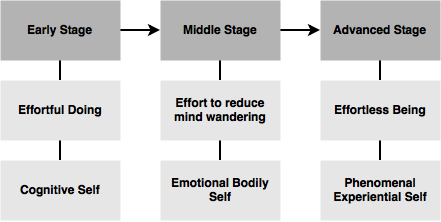
\includegraphics[width=0.8\textwidth]{figures/stages_of_meditation.png} 
	\caption{The three stages of meditation practice, describing how much effort one must use to get into the meditative state}
	\label{fig:meditation_stages}  
	\cite{Tang2017}
\end{figure}  \cite{Tang2017}

In the early stages more mental effort is required, here the dorsal lateral PFC and partial cortex are often involved and activated more. A stronger deactication in the DMN is shown to occur when using more effort. With lesser effort, the ACC and striatum will participate more. \cite{Tang2017}

The method of mindfulness meditation will not make the pain go away, but the patient will be able to deal with the pain easier, as mentioned, making the patient engage more in the treatment than focusing on and reeling on the medication. \cite{Jacob2016}
Very little mindfulness training can have an effect, the study by \cite{Zeidan2012} explaining an effect of training mindfulness meditation examined for 20 min sessions for 4 days of mindfulness meditation, but most studies conduct the experiments for a period of more than six weeks. \cite{Zeidan2012}

The neural mechanisms behind mindfulness meditation in reliving pain has been researched and in experiments where stimulating with nociceptive pain there has been shown an increase in activity areas of the PFC when meditating. Participants telling that they are able to feel the pain but able to deal with it better during meditation focusing on the breath. 
The same mechanisms working in analgsia is not the same as the mechanisms during meditation, why the two methods don't interfere with each other. \cite{Jacob2016}

The different areas of the brain show either a reduction or increase in activity when performing meditation. When practicing meditation the person trains the mind, and areas of specific regions will grow. \cite{Zeidan2012}

Examining long term meditators, the findings are a thicker gray matter in mid cingulate cortex and bilateral secondary somatosensory cortex, which are involved in pain related regions overlapping the functional effect. A correlation with the number of years practicing meditaiton and the mid cingulate was also found. This gives evidence to long lasting effects of meditation. \cite{Zeidan2012}


%More cognitive and emotional control causing better pain management.

%Activation of in brainareas responsible for encoding sensory aspects of nocious stimuli (insula, thalamus, mid-cingulate cortex). Decrease observed in regions involving emotion, memort and appraisal (medial-PFC, OFC, amygdala, caudate, hippocampus). \cite{Zeidan2012}

%reduced functional connectibity between DLPFC and mid-cingulate cortex during pain. The mental state whithin the meditators was that they where fully aware of the sensory properties of the stimuli, but still inhibiting apraisal, elaboration and emotional reactivity (decrease in brain areas, DLPFC, OFC, med-PFC, amygdala, hippocampus) \cite{Zeidan2012}
 